\chapter{引言}

这本书介绍的是一种在微波设备中起重要作用的电子管——行波管。

提起电子管,也许有人会想:“这种东西是不是比较落后?现代化的电子设备中,不是已经广泛应用晶体管、集成电路来代替电子管了吗?”

是的,在许多功率比较小、频率比较低的设备中,电子管已经基本上被晶体管所取代,但是在频率很高,功率较大的微微波设备中,目前电子管却还在起着重要的作用,不过他不是通常所见的普通电子管,而是在结构上和机理上都和普通电子管不同的特种电子管——微波电子管。行波管是微波电子管中的一种,它广泛地被用来作微波设备中的末级功率放大器。

行波管之所以在微波设备中能够得到广泛的应用,主要是由于在微波波段中,普通电子管已经不能胜任震荡、放大等重要任务了。为什么呢?

我们知道微波的频率很高,一般在300兆赫到300千兆赫\footnote{现在多认为300兆赫到3000千兆赫}之间,它的波长是在分米和毫米之间。在这样高的频率下,在普通电子管里电子从阴极飞到栅极和屏极的渡越时间已经和微波信号的周期可以比拟了,也就是说对于普通电子管里的垫电子渡越时间已经到了不能不考虑的程度了。必须要采用完全新的机理和结构的微波电子管才能解决这个问题。

微波的另一个特点是在通信中使用的频带很宽,带宽就意味着能够传送的信号多、能够传送各种频带很宽的信号。举例来说,一对铁线架空线路,最多只能传送几路电话,也就是说,铁线线路能够传送的频带很窄,对于频带较宽的信号是不能传送的。微波的频带很宽,我们知道,普通长波、中波、短波的频带宽度总合起来只有30兆赫,而微波的频带宽度达270千兆赫,几乎是长波、中波、短波合起来的频带宽度的10000倍!利用微波,不仅可以传送成千上万路电话,还可以传送频带很宽的电视信号。因而目前世界上大部分技术比较先进的国家里,50\%以上的长途电信都是利用微波通信来完成的。

微波的上述特点,对于微波接力通信设备中的元器件提出了一些新的要求。例如对微波接力通信设备末级功率放大器的要求是频带宽、增益高、输出功率较大(几瓦到十几瓦)、结构简单、工作稳定可靠、寿命长等。和其他微波电子管相比较,行波管能够较全面地满足上面这些要求,因此,目前的微波接力通信设备,几乎都采用行波管来作为它的末级功率放大器。

近年来,随着微波半导体器件的发展,出现了一些不用行波管的全固体化微波接力通信设备,但是,他们大多是用于微波支线的小容量微波设备。在大容量的微波干线中,由于微波半导体器件在工作频率、输出功率、增益、宽频带特性等方面还比不上行波管,因此行波管还占有很重要的地位。

我们知道,微波接力通信电路是由许多个微波站所组成的(例如一条1500公里长的微波电路,就需要建立30个微波站),每一个微波站中又有好多部微波收发信机(每一条微波电路由若干个微波通道组成),因此需要使用大量的行波管。很明显,它们的工作都应当十分可靠,因为一个微波通道中只要有一只行波管发生故障就会导致整个通道的通信全部中断或部分中断,引起严重的后果。

为了保证微波电路的正常运行,我们不但需要制造出质量优良的行波管,还有能够正确地使用和维护每一支行波管,使得它们都能稳定可靠的工作,因此了解熟悉行波管的工作原理、结构及其使用方法就是很必要的了。

微波接力通信中最常用的是输出功率为几瓦到十几瓦的所谓中小功率行波管,本书重点介绍的就是这类行波管。

实际上,最早的微波放大管不是行波管,而是双腔速调管,行波管可以说是在双腔速调管的基础上发展而来的。因此,在介绍行波管之前,我们有必要先简单地回顾一下双腔速调管。

我们知道在普通电子管中,我们是依靠栅极的静电控制作用来控制阳极电流,使它产生密度调制,出现与栅极信号波形相同的交变分量,从而在阳极得到放大了的交变电压的。在低频情况下,栅极的这个控制作用能够很好地发挥,其原因就在于在电子从阴极飞向阳极的这段渡越时间内,我们可以近似地认为栅极电压是不变的,因此它产生的电场就好像静电场那样作用于电子,静电控制作用就由此而得名。当频率升高时,虽然电子渡越时间并没有变,但是由于栅极信号周期大大缩短,致使在电子穿过电极空间的这段时间内,不能认为栅极电压是不变的了,因此栅极信号电压就不能很好地控制阳极电流使它按照栅极电压的波形而变化,也就是阳极电流的波形和栅极电压的波形之间产生了畸变,我们从阳极上得到的信号就是一个失真的信号。如果频率进一步升高,那么栅极的控制作用更差,电子的运动将变得很乱,阳流波形的畸变更为严重,以致整个管子的工作失效。由此可见,普通电子管在微波频率下不能工作的根本原因就是栅极静电控制作用的失灵。

双腔速调管采用了完全新的控制方法——速度调制方法,速调管的名称就是这样得来的。速度调制方法的要点是:先用交变电压对交变电子流进行微小的速度调制(即在电子流的直流速度分量上面叠加一个微小的交变速度分量),然后让这些电子在不受外加电场影响的漂移空间中做惯性运动。经过一段时间以后,不同速度的电子所走过的路程就不相同,于是,电子流的密度就慢慢地发生变化,最后就变成密度按照调制电压规律变化的电子流了(或叫做群聚电子流,关于群聚将在第二章中介绍),这种由速度调制转化为密度调制的方法,就叫做速度调制方法。

在速度调制方法中,电子在漂移空间中的渡越过程,是我们得到密度调制电子流所必需的,也就是说,我们是利用了电子渡越时间来实现速度调制向密度调制的转化的,因此,电子渡越时间是有利的,而在静电控制方法中,电子渡越时间则是有害的。

人们利用速度调制方法首先制成了双腔速调管,图\ref{ch1-1}是它的结构示意图。我们来分析一下双腔速调管中的物理过程。

\begin{figure}[phtb]
	\centering
	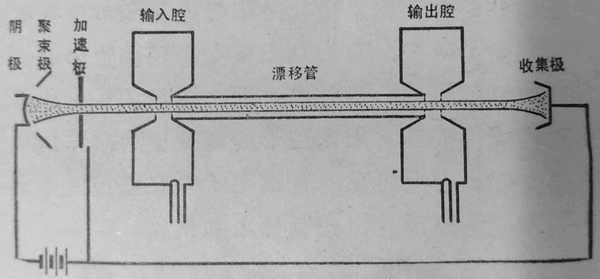
\includegraphics[width=\linewidth]{figure/ch1-1}
	\caption{双腔速调管示意图}
	\label{ch1-1}
\end{figure}

\begin{enumerate}
	\item 高速电子流胡产生。阴极发射出来的电子,在高达几千伏的阳极电压加速下得到了足够大的速度,因而具备了足够大的动能。与普通电子管中的阳极不同,速调管中的阳极是中心开孔的,他只对电子进行加速而不截获电子。这里阴极、聚束极和阳极组成了一个小部件,叫做电子枪。从电子枪中射出的电子流是一个高速的均匀电子流,下一步就将对它进行速度调制了。显而易见,高速粒子流的动能是直流电源给它的。
	\item 对高速电子流进行密度调制。这个过程是在输入谐振腔和漂移管中完成的。输入交变信号在谐振腔的隙缝处产生交变电场,当高速电子流穿过输入腔隙缝时,交变电场就要对它产生作用,使它的速度受到调制。漂移管实际上就是一根中空的金属圆管,它屏蔽了外界的一切电磁场,为电子流制造了一个无场空间,于是电子流就在里面做惯性运动,逐渐群聚,最后变成和输入信号波形相同的密度调制电子流。这个过程也就是速度调制方法的实现过程。
	\item 密度调制电子流(即群聚电子流)与输出谐振腔隙缝处的交变电场相互作用并把自己的能量交给高频场(以后,我们习惯把微波交变电磁场叫作高频场或微波信号),使它得到放大,于是,在输出腔就可以得到放大了的微波信号。
	
	为什么群聚电子流与高频场相互作用的结果是前者把能量交给后者使后者增强而不是相反呢?分析表明,当群聚电子流穿过输出腔隙缝时,大部分电子是在减速高频场瞬间穿过的,只有小部分电子是在加速高频场瞬间穿过的。我们知道,电子在加速电场中运动时将从电场中得到能量,变成自己附加的动能,因而速度加快,而电场的能量就要减小,电场减弱;电子在减速电场中运动时,将把自己的部分动能交给电场,使电场能量增大,电场增强,而电子则由于失去了部分动能,因而速度减小。因此大部分电子流在减速高频场瞬间穿过输出腔隙缝的结果就将使群聚电子流有净的能量交给高频场,使它得到增强,最后得到放大的高频信号。这个过程是电子流把自己从直流电源中得来的部分动能交给高频电场使之增强的过程,因此是双腔速调管中最本质的过程。	
	\item 收集工作完毕的电子流。这个任务由收集极来完成,从输出腔隙缝穿出的电子流带着剩余的动能打上收集极并全部变为热能。
\end{enumerate}

从上面所分析的四个物理过程中,我们可以得出一个重要的结论:双腔速调管是借助于交变电子流来实现直流电场和高频电场之间的能量转换,从而使高频信号得到放大的一种器件。实际上,这个结论对于一切用于放大的电子管都是适合的。下面,我们将看到,在行波管中也存在着相同的四个物理过程(但实现这四个物理过程的方法有所不同),双腔速调管中的群聚和能量交换这两个概念同样也是行波管中最基本的概念,因此,上面的分析对于我们了解行波管的工作原理是有帮助的。

双腔速调管虽然可以对微波信号进行放大,但是它却不能很好地满足微波通信的要求,其主要原因就是双腔速调管的频带窄。在第二章中,我们将分析双腔速调管频带窄的原因,并由此导出行波管的工作原理。
